% template adapted from https://github.com/jgm/pandoc-templates/blob/master/default.latex

%%% STYLE %%%
\documentclass[12pt,]{article}

%%% PACKAGES %%%

% fonts
\usepackage{lmodern}

% pdf
\usepackage{pdfpages}

% formulae
\usepackage{amssymb,amsmath}
\usepackage{ifxetex,ifluatex}
\usepackage{fixltx2e}
\usepackage[T1]{fontenc}
\usepackage[utf8]{inputenc}

% Tables
% pacakges for kableextra
\usepackage{booktabs}
\usepackage{longtable}
\usepackage{array}
\usepackage{multirow}
\usepackage{wrapfig}
\usepackage{float}
\usepackage{colortbl}
\usepackage{pdflscape}
\usepackage{tabu}
\usepackage{threeparttable}
\usepackage{threeparttablex}
\usepackage[normalem]{ulem}
\usepackage{makecell}
\usepackage{xcolor}
% Fix footnotes in tables (requires footnote package)
\IfFileExists{footnote.sty}{\usepackage{footnote}\makesavenoteenv{long table}}{}

% graphics
\usepackage{graphicx,grffile}
\makeatletter
\def\maxwidth{\ifdim\Gin@nat@width>\linewidth\linewidth\else\Gin@nat@width\fi}
\def\maxheight{\ifdim\Gin@nat@height>\textheight\textheight\else\Gin@nat@height\fi}
\makeatother
\setkeys{Gin}{width=\maxwidth,height=\maxheight,keepaspectratio}

% indent
\IfFileExists{parskip.sty}{%
\usepackage{parskip}
}{% else
\setlength{\parindent}{0pt}
\setlength{\parskip}{6pt plus 2pt minus 1pt}
}

% prevent overfull lines
\setlength{\emergencystretch}{3em}  
\providecommand{\tightlist}{%
\setlength{\itemsep}{0pt}\setlength{\parskip}{0pt}}

\setcounter{secnumdepth}{0}

% set default figure placement to htbp
\makeatletter 
\def\fps@figure{htbp}
\makeatother

% set default table placement to htbp
\makeatletter 
\def\fps@table{htbp}
\makeatother

% code highlights

% hyperlinks
\IfFileExists{upquote.sty}{\usepackage{upquote}}{}
\IfFileExists{microtype.sty}{%
\usepackage[]{microtype}
\UseMicrotypeSet[protrusion]{basicmath} % disable protrusion for tt fonts
}{}
\PassOptionsToPackage{hyphens}{url} % url is loaded by hyperref
\usepackage[unicode=true]{hyperref}
\definecolor{maroon}{cmyk}{0, 0.87, 0.68, 0.32}
\hypersetup{
      pdfborder={0 0 0},
      breaklinks=true}
\urlstyle{same} % don't use monospace font for urls

% geometry
\usepackage[left=2.5cm,right=2.5cm,top=2.5cm,bottom=2.5cm]{geometry}
\renewcommand{\baselinestretch}{1.1}

% Bibliography
\usepackage{natbib}
\bibliographystyle{plainnat}

% SuppMat
\renewcommand{\figurename}{Figure S}
\renewcommand{\tablename}{Table S}
\renewcommand{\contentsname}{Supplemental content}
\renewcommand{\listtablename}{Supplemental tables}
\renewcommand{\listfigurename}{Supplemental figures}

% header
\usepackage{fancyhdr}
\pagestyle{fancy}
\fancyhead[H]{} 
\renewcommand{\headrulewidth}{0pt}
\renewcommand{\footrulewidth}{0pt}
\setlength\headheight{80.0pt}
\addtolength{\textheight}{-80.0pt}
\chead{
\includegraphics[width=\textwidth]{template/molecol.png}}

%%% BODY %%%
\begin{document}

\begin{center}
  \normalsize{\textbf{Supplemental Information for:}} \\
  \vspace{5mm}
  \large{\textbf{Topography drives microgeographic adaptations among closely-related species of two tropical tree species complexes}} \\
  \vspace{5mm}
  \normalsize{Sylvain Schmitt, Niklas Tysklind, Bruno Herault, Myriam Heuertz} \\
  \tableofcontents
  \listoftables
  \listoffigures
\end{center}

\newpage

\hypertarget{model-s1-stan-code-for-the-bayesian-inference-of-the-animal-model.}{%
\section{Model S1: Stan code for the bayesian inference of the animal model.}\label{model-s1-stan-code-for-the-bayesian-inference-of-the-animal-model.}}

\begin{verbatim}
data {
  int<lower=0>  N ; // # of individuals
  int<lower=0>  P ; // # of populations
  real y[N] ; // phenotype
  int<lower=1, upper=P> population[N] ; // populations
  cov_matrix[N] K ; // kinship covariance matrix
}
transformed data{
  matrix[N, N] A = cholesky_decompose(K) ; // cholesky-decomposed kinship
  real Vy = variance(log(y)) ;
}
parameters {
  vector<lower=0>[P] mu ; // intercept
  vector[N] epsilon ; // genotypic noise
  real<lower=0, upper=sqrt(Vy)> sigma ; // genetic variance
}
transformed parameters {
  real<lower=0> Vp = variance(log(mu[population])) ; // population variance
  real Vr = square(sigma) ;
  real Vg = Vy - Vp - Vr ;
  vector[N] alog = sqrt(Vg)*A*epsilon ;
}
model {
  y ~ lognormal(log(mu[population]) + alog, sigma) ;
  epsilon ~ std_normal() ;
  mu ~ lognormal(0, 1) ;
  sigma ~ normal(0, 1) ;
}
\end{verbatim}

\newpage

\begin{figure}[H]

{\centering 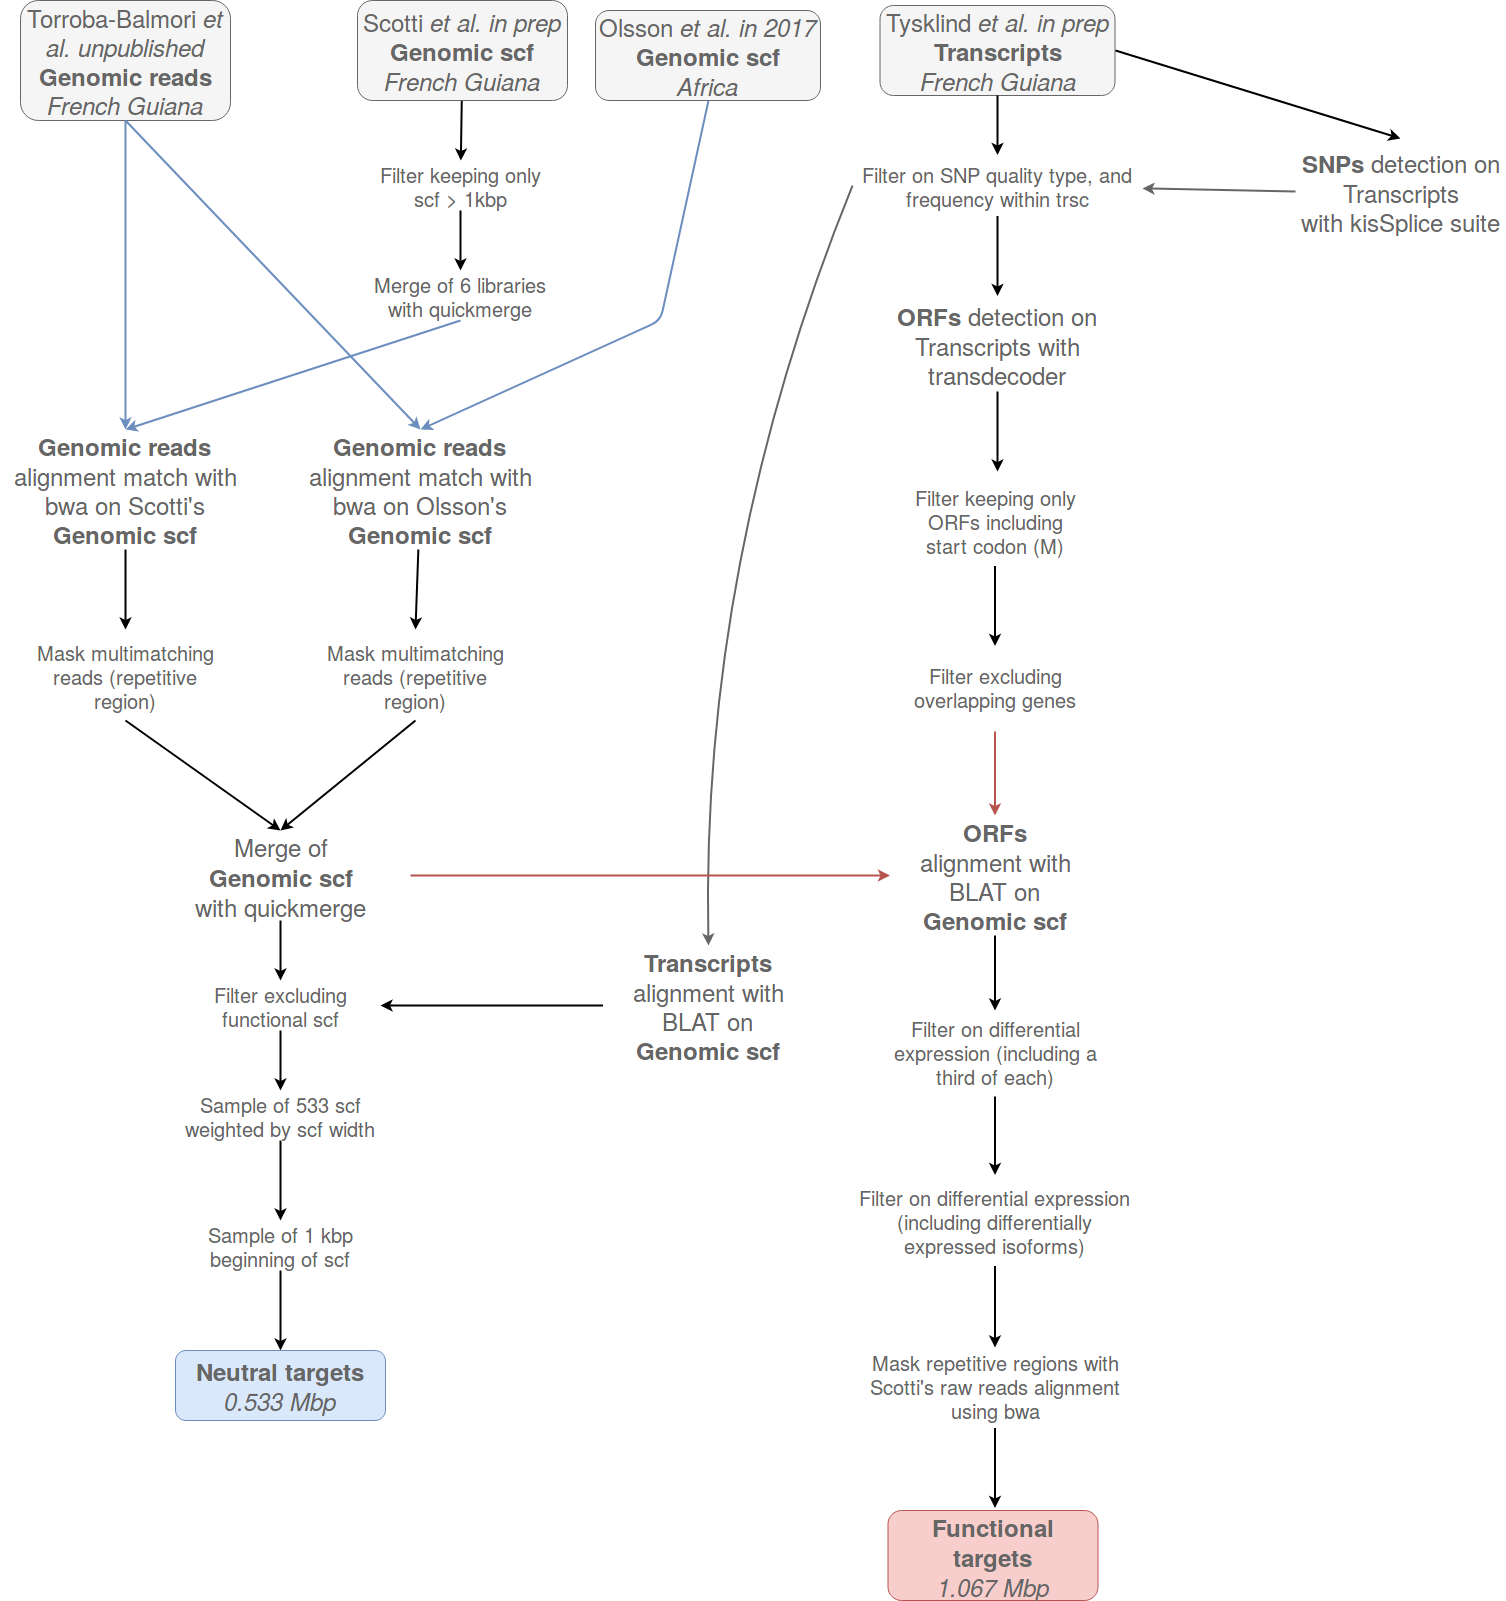
\includegraphics[width=\linewidth]{figures/Symcapture} 

}

\caption{Scheme of target selection for the capture experiment of \emph{Symphonia globulifera} as described in the manuscript.}\label{fig:symcapture}
\end{figure}

\newpage

\begin{figure}[H]

{\centering 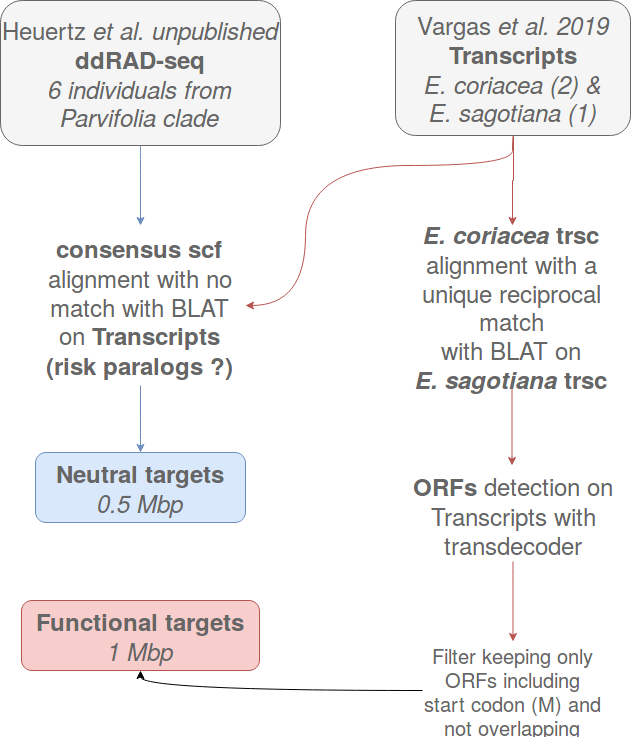
\includegraphics[width=\linewidth]{figures/Parvicapture} 

}

\caption{Scheme of target selection for the capture experiment of \emph{Eschweilera} clade \emph{Parvifolia} as described in the manuscript.}\label{fig:parvicapture}
\end{figure}

\newpage

\begin{figure}[H]

{\centering \includegraphics{TopoSuppMatMolEcol_files/figure-latex/libmiss-1} 

}

\caption{SNP abundance per library rank for raw data of \emph{Eschweilera} clade \emph{Parvifolia}. Dashed lines represent tested filters.}\label{fig:libmiss}
\end{figure}

\newpage

\begin{figure}[H]

{\centering \includegraphics{TopoSuppMatMolEcol_files/figure-latex/snpmiss-1} 

}

\caption{Library abundance per SNP rank for library-filtered data of \emph{Eschweilera} clade \emph{Parvifolia}. Dashed lines represent tested filters.}\label{fig:snpmiss}
\end{figure}

\newpage

\begin{figure}
\centering
\includegraphics{TopoSuppMatMolEcol_files/figure-latex/outgroup-1.pdf}
\caption{\label{fig:outgroup}Outgroup detection with individual clustering in the genomic principal component analysis (gPCA) in two groups using K-means for every filter.}
\end{figure}

\newpage

\begin{figure}
\centering
\includegraphics{TopoSuppMatMolEcol_files/figure-latex/admixtureSympoCV-1.pdf}
\caption{\label{fig:admixtureSympoCV}Cross-validation for the clustering of \emph{Symphonia} individuals. Y axis indicates corss-validation mean error, suggesting that 2 or 3 groups represent the best Paracou individuals structure.}
\end{figure}

\newpage

\begin{figure}
\centering
\includegraphics{TopoSuppMatMolEcol_files/figure-latex/admixtureSympo-1.pdf}
\caption{\label{fig:admixtureSympo}Population structure of \emph{Symphonia} individuals from K=2 to K=10.}
\end{figure}

\newpage

\begin{figure}
\centering
\includegraphics{TopoSuppMatMolEcol_files/figure-latex/introgress-1.pdf}
\caption{\label{fig:introgress}Population structure with hybrid index (black line and white interval confidence) and admixture coefficient (vertical bars).}
\end{figure}

\newpage

\begin{figure}
\centering
\includegraphics{TopoSuppMatMolEcol_files/figure-latex/bayescanOutliers-1.pdf}
\caption{\label{fig:bayescanOutliers}Species-specific SNPs for \emph{Symphonia} individuals detected with bayescan.}
\end{figure}

\newpage

\begin{longtable}[]{@{}lrrr@{}}
\caption{\label{tab:kmeansConfusion}Confusion matrix (percentage) between genetic cluster and botanical identification for \emph{Eschweilera} clade \emph{Parvifolia}.}\tabularnewline
\toprule
Species & E. coriacea cluster & E. decolorans cluster & E. sagotiana cluster\tabularnewline
\midrule
\endfirsthead
\toprule
Species & E. coriacea cluster & E. decolorans cluster & E. sagotiana cluster\tabularnewline
\midrule
\endhead
E. coriacea & 65 & 8 & 13\tabularnewline
E. decolorans & 15 & 77 & 7\tabularnewline
E. sagotiana & 20 & 16 & 80\tabularnewline
\bottomrule
\end{longtable}

\bibliography{/home/sylvain/Documents/Bibliography/library.bib}

\end{document}
